\documentclass[xcolor={dvipsnames}]{beamer}
\usetheme{Malmoe}
\usecolortheme{spruce}
\setbeamercolor{item}{fg=PineGreen}
\setbeamertemplate{itemize item}[square]
\setbeamertemplate{itemize subitem}[triangle]
\setbeamertemplate{itemize subsubitem}[square]
\setbeamertemplate{itemize/enumerate subbody begin}{\vspace{0.5em}}

\usepackage{amsmath,amsthm,amssymb}
\usepackage{mathtools}
\usepackage{mathrsfs}
\usepackage{physics}
\usepackage{graphicx}
\usepackage{caption}
\usepackage{animate}

\let\olditemize=\itemize 
\let\endolditemize=\enditemize 
\renewenvironment{itemize}{\olditemize \itemsep=.5em }{\endolditemize}

\graphicspath{ {./images/} }

\newcommand{\avg}[1]{\left<#1\right>}

%Information to be included in the title page:
\title{Nash Equilibrium of the LUPI Game}
\subtitle{Direct Calculation and Simulation via Genetic Algorithm}
\author{Sean Ericson}
\institute{UO}
\date{Theory meeting, April 25, 2024}
\titlegraphic{
\includegraphics[scale=0.10]{seal.png}}

\begin{document}

\frame{\titlepage}

\begin{frame}{The Lowest Unique Positve Integer Game}
\begin{itemize}
    \item<1-> There are $N$ players.
    \item<2-> Each player selects an integer $1 \leq i \leq N$.
    \item<3-> The player that selected the lowest unique integer wins a point.
    \item<4-> If no player selects a unique integer, no one wins.
\end{itemize}
\end{frame}

\begin{frame}{Nash Equilibrium}
\begin{itemize}
    \item<1-> Property of multiplayer competitive games
    \item<2-> All players strategies are public (or at least inferable)
    \item<3-> The set of players' strategies is in a NE when no player can improve their expected performance by changing only their own strategy
    \item<4-> Often not optimal
\end{itemize}
\end{frame}

\begin{frame}{Example: Traffic (Braess's Paradox)}
\begin{figure}
    \centering
    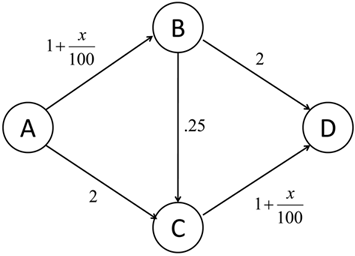
\includegraphics[scale=1.5]{Nash_graph_equilibrium.png}
\end{figure}
\begin{align*}
    \onslide<1->{&t_{ABD} = t_{ACD} = 3\;\text{hr} + 0.01\;\frac{\text{hr}}{\text{car}} \\}
    \onslide<2->{&t_{ABCD} = 2.25\;\text{hr} + 0.02\;\frac{\text{hr}}{\text{car}} \\}
    \onslide<3->{&\text{NE: } t_{ABD} = t_{ACD} = t_{ABCD} = 3.75 \\}
    \onslide<4->{&\text{Optimum: } t_{ABD} = t_{ACD} = 3.5,\quad t_{ABCD} = 3.25 \\}
\end{align*}
\end{frame}

\begin{frame}{NE Calculation for LUPI}
\begin{itemize}
    \item<1-> Let players $1,\cdots,(N-1)$ have strategy $\vec{p} = (p_1, p_2, \dots, p_n)$, and denote the $N^\text{th}$ player's strategy as $\vec{\pi}$.
    \item<2-> ``Generating function'' for the possible choices of the $(N-1)$ players:
    \onslide<3->{ \[ Z_0 = \left(\sum_{i=1}^N p_i\right)^{N-1} \]}
    \item<4-> E.g. $N=3\; \implies Z_0 = p_1^2 + p_2^2 + 2(p_1p_2 + p_1p_3 + p_2p_3)$
    \item<5-> Note that Coef[$Z_0$; $p_{i_1}^{n_1}p_{i_2}^{n_2}\dots p_{i_k}^{n_k}$] is the number of ways that the $(N-1)$ players can pick the number $i_1$ $n_1$ times, etc. 
\end{itemize}
\end{frame}

\begin{frame}{NE Calculation for LUPI (cont.)}
\begin{itemize}
    \item<1-> Cases in which exactly one of the ($N-1$) players picked the number 1 are those terms with exactly one factor of $p_1$.
    \item<2-> Write $Z_0$ as a polynomial in only $p_1$:
    \onslide<3->{\[ Z_0 = A_0(p_2,\cdots,p_n) + A_1(p_2,\cdots,p_n)p_1 + \cdots \]}
    \item<4-> The term
    \[ A_1p_1 = \dv{Z_0}{p_1}\bigg\rvert_{p_1=0}p_1 \]
    contains exactly the cases in question.
\end{itemize}
\end{frame}

\begin{frame}{NE Calculation for LUPI (cont.)}
\alert{Operator Time}
\begin{itemize}
    \item<1-> For an arbitrary polynomial $Q$ of $p_1,\cdots,p_n$, define
    \begin{itemize}
        \item<2-> $D_i[Q] \coloneqq \dv{Q}{p_i}$
        \item<3-> $E_i[Q] \coloneqq Q\big\rvert_{p_i=0}$ 
        \item<4-> $L_i[Q] \coloneqq p_i(E_i\circ D_i)[Q]$
    \end{itemize}
    \item<5-> Clearly,
    \[ \comm{p_i}{p_j} = \comm{D_i}{D_j} = \comm{E_i}{E_j} = \comm{D_i}{E_j} = \comm{p_i}{E_j} = 0, \]
    and 
    \[ \comm{D_i}{p_j} = \delta_{ij} \]
\end{itemize}
\end{frame}

\begin{frame}{NE Calculation for LUPI (cont.)}
\alert{Quick Facts About $L_i$}
\begin{itemize}
    \item<1-> $L_i[ap_j^n] = ap_i\delta_{1,n}$
    \item<2-> $L_i[aQ_1 + bQ_2] = aL_i[Q_1] + bL_i[Q_2]$
    \item<3-> $L_i[L_i[Q]] = L_i[Q]$
    \item<4-> $\comm{L_i}{L_j} = 0$
    \item<5-> $\comm{E_i}{L_j} = 0$*
\end{itemize}
\end{frame}

\begin{frame}{NE Calculation for LUPI (cont.)}
\begin{itemize}
    \item<1-> So, the ways in which exactly one of the $(N-1)$ players can select 1 are given by 
    \[ L_1[Z_0]. \]
    \item<2-> Then, the probability that \textit{no} unique person of the $(N-1)$ players selects 1 is give by
    \begin{align*}
        Z_1 &\coloneqq Z_0 - L_1[Z_0]  \\
        &= \left(\sum_{i=1}^N p_i\right)^{N-1} - (N-1)p_1\left(\sum_{i=2}^N p_i\right)^{N-2}.
    \end{align*}
    \item<3-> Continuing, cases excluding unique selection of 1 \textit{and} 2 are given by
    \[ Z_2 = Z_1 - L_2[Z_1]. \]
\end{itemize}
\end{frame}

\begin{frame}{NE Calculation for LUPI (cont.)}
\begin{itemize}
    \item<1-> We then have the recurrence relation
    \[ Z_k = Z_{k-1} - L_k[Z_{k-1}] \]
    \item<2-> It's fairly straightforward to show that, for all $i<j$, $L_i[Z_j] = 0$
    \item<3-> Then, we can write the $Z_k$ as
    \[ Z_k = \left[\prod_{i=1}^k (1 - L_i)\right]Z_0 \]
\end{itemize}
\end{frame}

\begin{frame}{NE Calculation for LUPI (cont.)}
\alert{Putting it all together..}
\begin{itemize}
    \item<1-> The probability for the $N^\text{th}$ player to win by selecting the number $i$ is
    \begin{itemize}
        \item<2-> the probability for the player to pick $i$, $\pi_i$,
        \item<3-> multiplied by the probability that 
        \begin{itemize}
            \item<4-> there are no winners among the $(N-1)$ other players, and
            \item<5-> none of the $(N-1)$ players picked $i$. 
        \end{itemize}
    \end{itemize}
    \item<6-> That is, $c_i = \pi_iE_i[Z_i]$
    \item<7-> The $N^\text{th}$ player's expected performance is then
    \[ W(\vec{\pi}; \vec{p}) = \sum_{i=1}^N c_i\pi_i \]
\end{itemize}
\end{frame}

\begin{frame}{NE Calculation for LUPI (cont.)}
\alert{Putting it all together..(cont.)}
\begin{itemize}
    \item<1-> Under the Nash equilibrium, we have that
    \[ \pdv{\vec{\pi}}W(\vec{\pi}; \vec{p}_\text{NE}) = 0. \]
    \item<2-> This can only occur if all $c_i = c_0$ for some $c_0$.
    \item<3-> We therefore have a system of $N$ equations,
    \[ c_i(\vec{p}) = c_0 \quad 1 \leq i \leq N, \]
    with $N$ degrees of freedom ($(N-1)$ in $\vec{p}$, and $c_0$).
\end{itemize}
\end{frame}

\begin{frame}{NE LUPI Distributions}
\begin{itemize}
    \item<1-> For $N=3$, the system of equations in analytically solvable, and we find
    \begin{align*}
        c_0 &= 28 - 16\sqrt{3} \\
        c_1 &= 2\sqrt{3} - 3 \\
        c_2 = c_3 &= 2 - \sqrt{3}
    \end{align*}
\end{itemize}
\end{frame}

\begin{frame}{Distributions (cont.)}
\begin{columns}[t]
    \column{.5\textwidth}
    \begin{figure}
        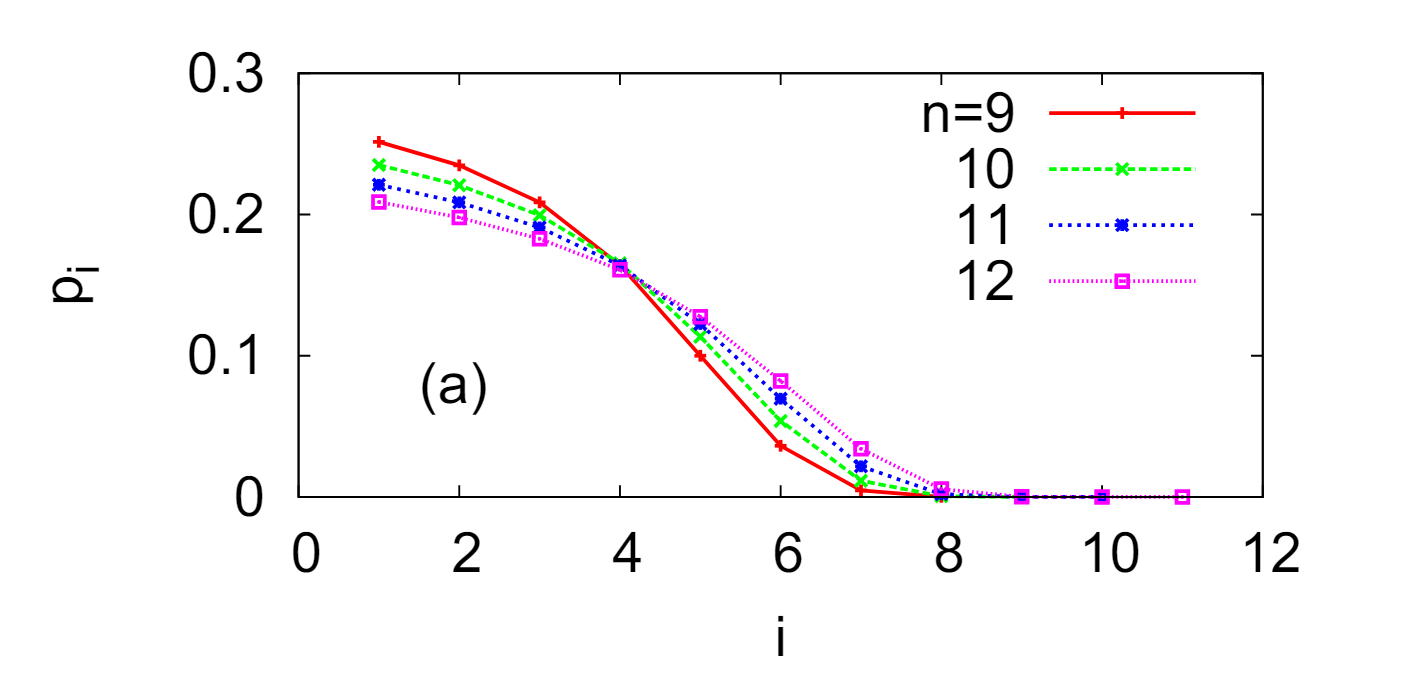
\includegraphics[scale=0.25]{paper.PNG}
    \end{figure}
    \vspace{-2em}
    \begin{figure}
        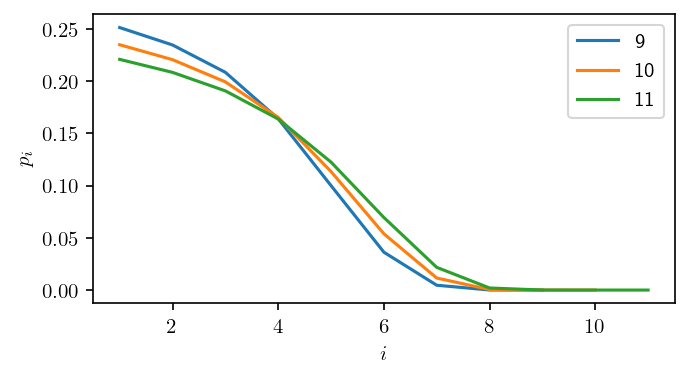
\includegraphics[scale=0.5]{mine.PNG}
    \end{figure}

    \column{.5\textwidth}
    \begin{figure}
        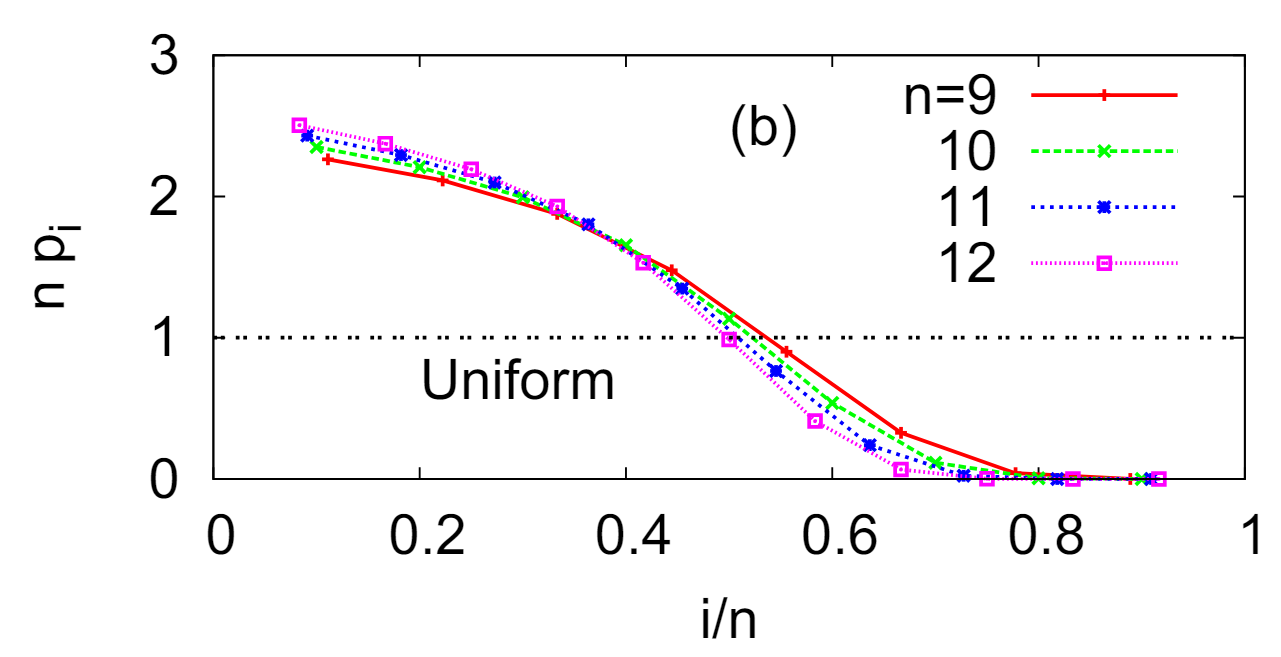
\includegraphics[scale=0.25]{paper_scaled.PNG}
    \end{figure}
    \vspace{-2em}
    \begin{figure}
        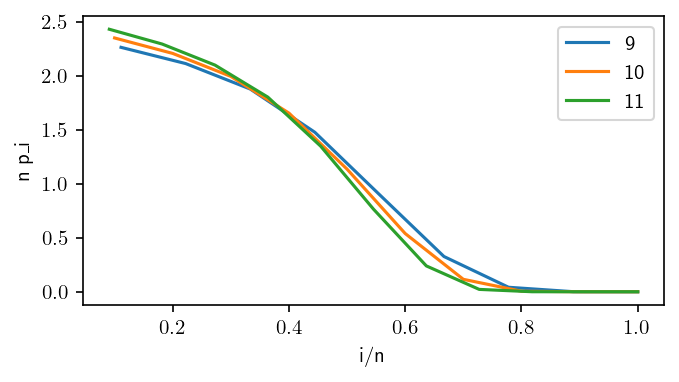
\includegraphics[scale=0.5]{mine_scaled.PNG}
    \end{figure}
\end{columns}
\end{frame}

\end{document}